\documentclass[xcolor=table, aspectratio=169, bigger]{beamer}

\usepackage{shyne}

% Theme settings
\setbeamertemplate{navigation symbols}{}

\usetheme{Madrid}
\usefonttheme{structurebold}
\usefonttheme[onlymath]{serif}

\AtBeginSection[]
{ 	\begin{frame}{}

	{
	\usebeamerfont{frametitle}
	\begin{beamercolorbox}
		[wd={\textwidth}, center, sep=.2in, rounded=true, shadow=true]
		{frametitle}
	Week \thesection\\  \secname 
	\end{beamercolorbox}
	}
	
	\end{frame} 
}

\AtBeginSubsection[]
{ 	\begin{frame}{}

	{
	\usebeamerfont{frametitle}
	\begin{beamercolorbox}
		[wd={\textwidth}, center, sep=.2in, rounded=true, shadow=true]
		{frametitle}
	Section \thesection .\thesubsection\\  \subsecname 
	\end{beamercolorbox}
	}
	
	\end{frame} 
}

\title[Week 11]{Stat 201: Statistics I\\Week 11 }
\author[M. Shyne]{}
\institute[Metro State]{
\includegraphics[width=1.75in]{../images/metro_logo}}
\date[4/21/2019]{
\\ \bigskip \bigskip 
\includegraphics[width=.4in]{../images/cc_big}}


\begin{document}
\frame{\titlepage}

%
% Chapter 11
%
\setcounter{section}{10}
\section{Correlation and Regression}

%%%%%%%%%%
\begin{frame}{Comparing samples from two populations}
\begin{exampleblock}{Example}
Consider the following data:\\
\smallskip
{\centering
\begin{tabular}{c | c c c c c c}
X & 83 & 85 & 66 & 89 & 96 & 78\\
\hline
Y & 90 & 90 & 66 & 86 & 99 & 85
\end{tabular}
\par}
\medskip
How should this data be analyzed? It depends on the context of the data or what the data represents.
\begin{itemize}
\pause\item Suppose the data is test scores from two different statistics classes.
\begin{itemize}
\pause\item One possible analysis would be a two-sample t-test comparing the mean test scores from each class.
\end{itemize}
\pause\item Suppose the data are scores from the midterm and the final for one set of students.
\begin{itemize}
\pause\item One possible analysis would be a matched pairs t-test comparing the mean  difference between the midterm and the final for each student.
\end{itemize}
\end{itemize}
\end{exampleblock}
\end{frame}

%%%%%%%%%%
\begin{frame}{Comparing samples from two populations, cont.}
\begin{exampleblock}{Example}
\smallskip
{\centering
\begin{tabular}{c | c c c c c c}
X & 83 & 85 & 66 & 89 & 96 & 78\\
\hline
Y & 90 & 90 & 66 & 86 & 99 & 85
\end{tabular}
\par}
\medskip
\begin{itemize}
\item Suppose X is a students score on the statistics final and Y is that students yearly salary, in thousands of dollars, a year later.
\begin{itemize}
\pause\item It doesn't really make sense to compare means. The two samples represent entirely different kinds of data. There is no meaningful way to compare means.
\pause\item It is useful to examine the association between the data. Is a higher test score associated with a higher salary? Or are the samples independent, values of one having no effect on values of the other?
\end{itemize}
\end{itemize}

\end{exampleblock}
\end{frame}

%%%%%%%%%%
\begin{frame}{Scatterplots}
\begin{block}{}
A \bt{scatterplot} is a useful way to visually examine paired data. Every data pair is represented by one point in the plot.
\end{block}
\bigskip

{\centering
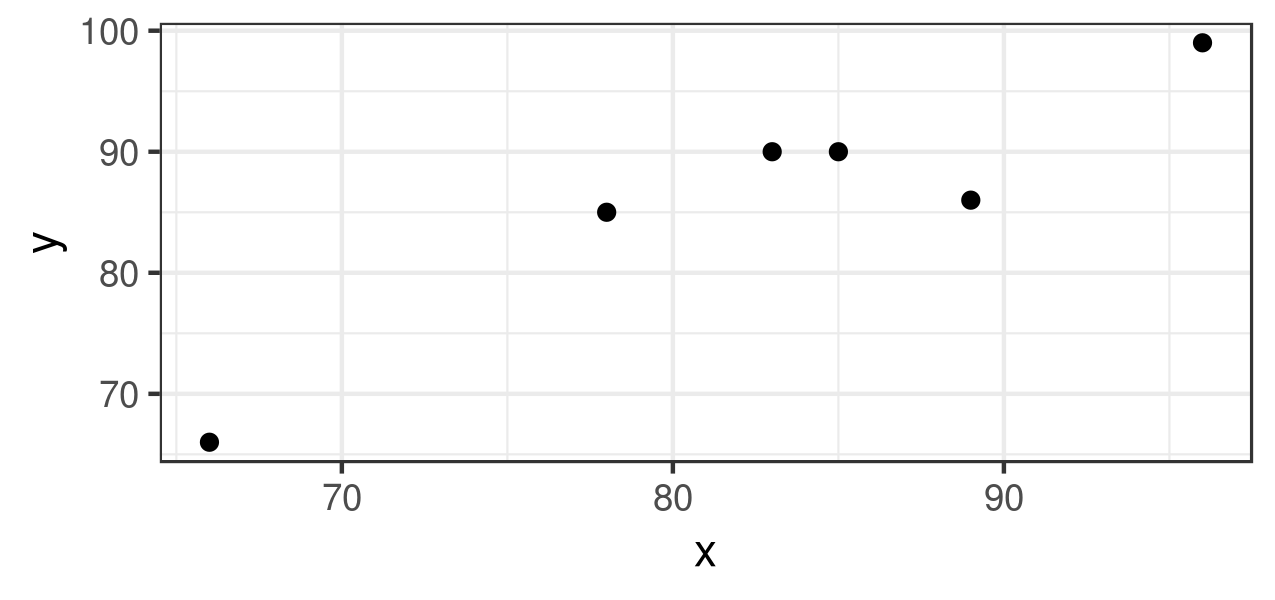
\includegraphics[width=4.25in]{../images/wk11_xy_scatter}
\par}

\end{frame}


%
% Section 11.1
%
\subsection{Correlation}

%%%%%%%%%%
\begin{frame}{Correlation}
\begin{block}{}
\bt{Correlation} is the measure of how strongly associated values of paired data are with each other.\\
\pause\medskip
\bt{Linear correlation} is the measure of how strong of a linear relationship (along a straight line)  values of paired data have with each other. 
\begin{itemize}
\pause\item A positive correlation indicates that as one value in a pair increases the other will tend to increase.
\pause\item A negative correlation indicates that as one value in a pair increases the other will tend to decrease.
\pause\item No correlation indicates that the two values of a pair have no relationship with each other. They are independent.
\end{itemize}
\end{block}
\end{frame}

%%%%%%%%%%
\begin{frame}{Correlation coefficient}
\begin{block}{}
The sample \bt{correlation coefficient}, denoted as $r$, is the numeric value for the strength of linear correlation between values of paired data.
\begin{itemize}
\pause\item $r$ is always between -1 and 1
\pause\item When $r=1$, the samples have perfect positive correlation
\pause\item When $r=-1$, the samples have perfect negative correlation
\pause\item When $r=0$, the samples are perfectly independent
\pause\item Most samples will have some other value for $r$. 
\pause\item The order of the values, i.e. $(x,y)$ vs. $(y,x)$, have no effect of the value of $r$.
\pause\item The units of the values also have no effect on $r$. A correlation on height will be the same whether it is measured in inches, feet or meters, for example.
\end{itemize}
\end{block}
\end{frame}

%%%%%%%%%%
\begin{frame}{Perfect correlation}

{\centering
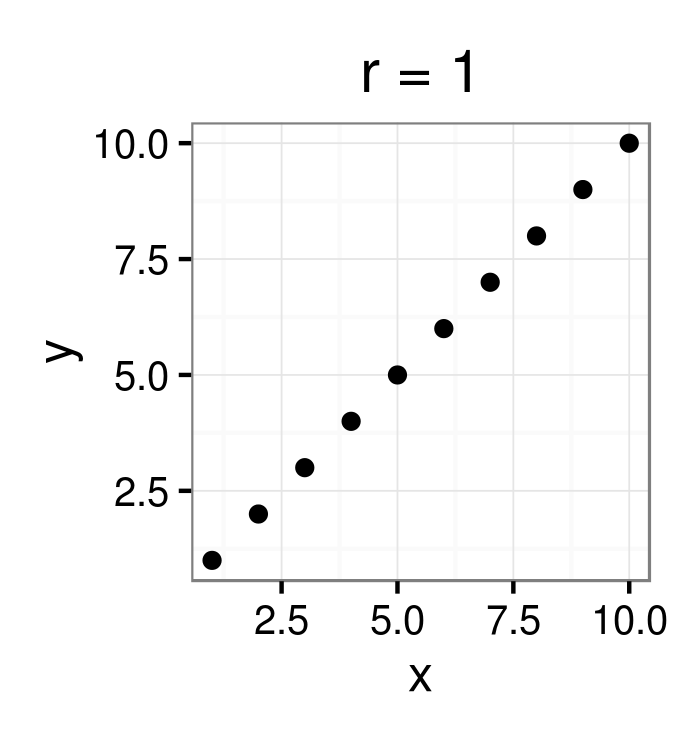
\includegraphics[width=2.25in]{../images/ch10_cor_pos1}
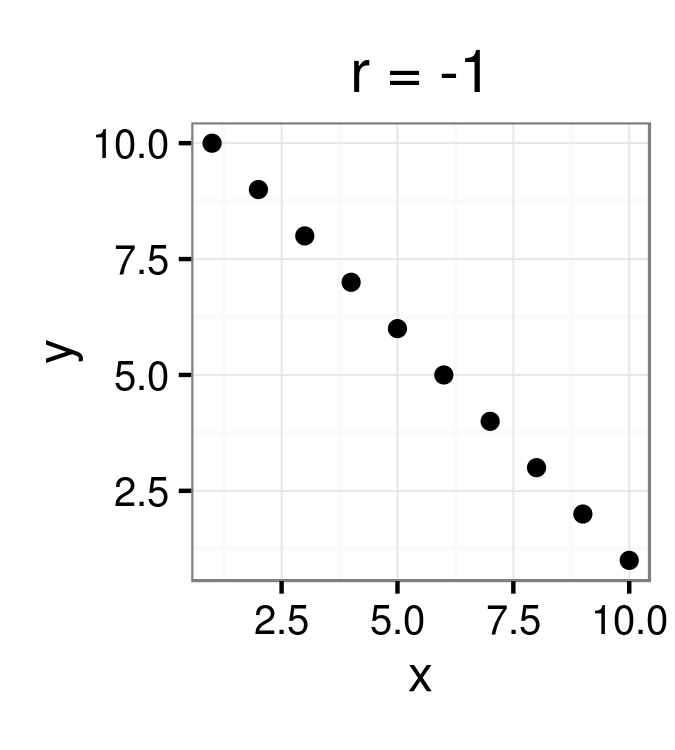
\includegraphics[width=2.25in]{../images/ch10_cor_neg1}
\par}
\end{frame}

%%%%%%%%%%
\begin{frame}{Perfect correlation, cont.}

{\centering
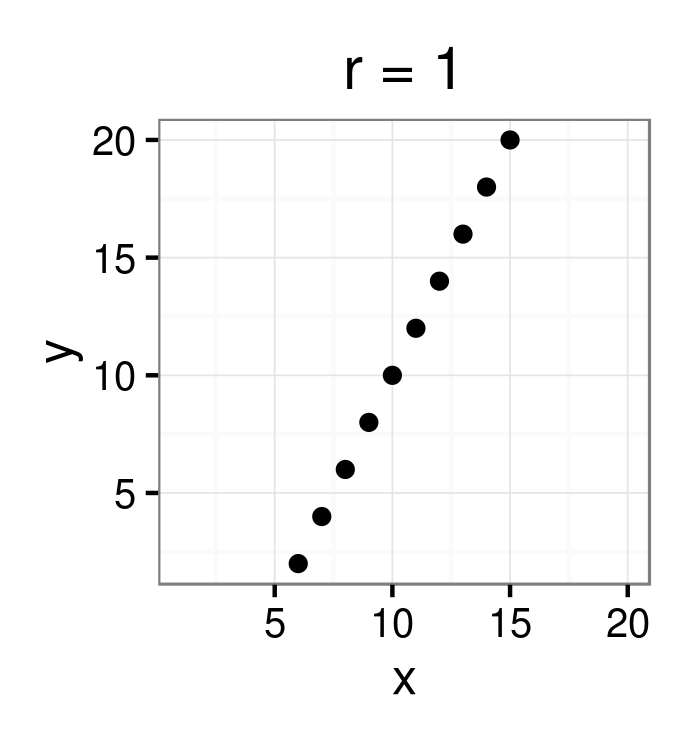
\includegraphics[width=2.25in]{../images/ch10_cor_pos2}
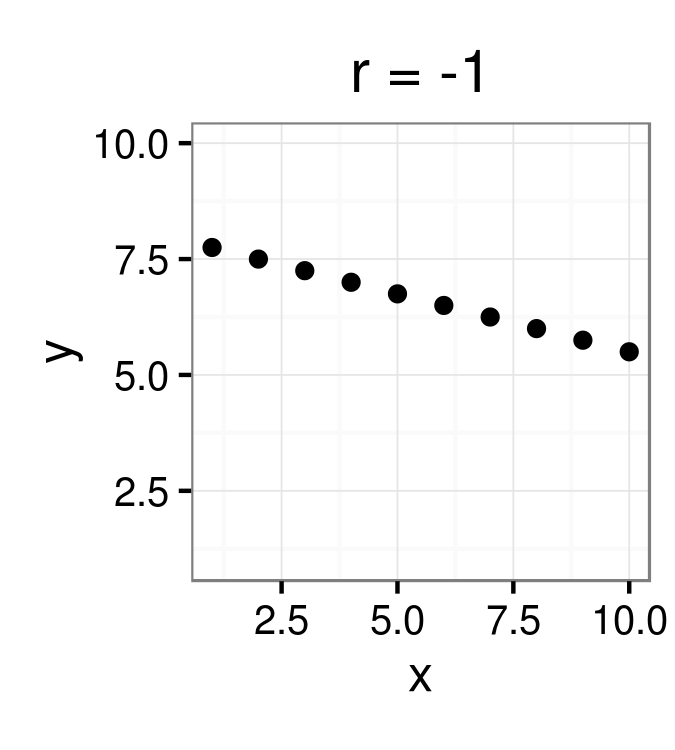
\includegraphics[width=2.25in]{../images/ch10_cor_neg2}
\par}
\end{frame}

%%%%%%%%%%
\begin{frame}{Zero correlation}

{\centering
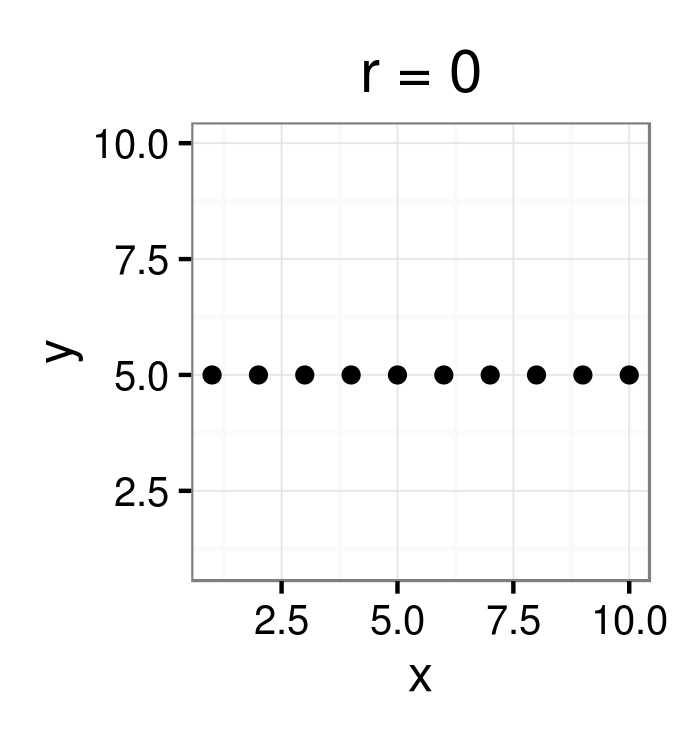
\includegraphics[width=2.25in]{../images/ch10_cor_zero}
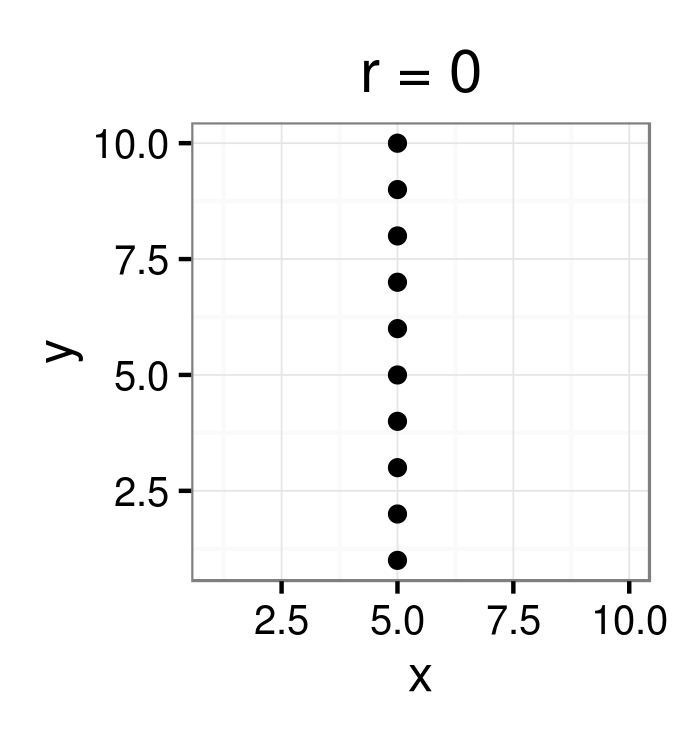
\includegraphics[width=2.25in]{../images/ch10_cor_zerox}
\par}
\end{frame}

%%%%%%%%%%
\begin{frame}{Non-linear correlation}

{\centering
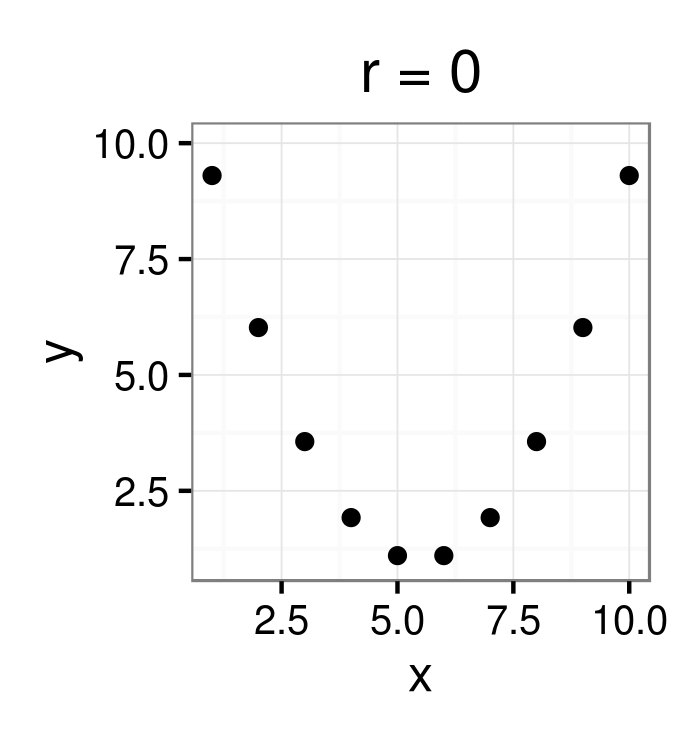
\includegraphics[width=2.25in]{../images/ch10_cor_para}
\pause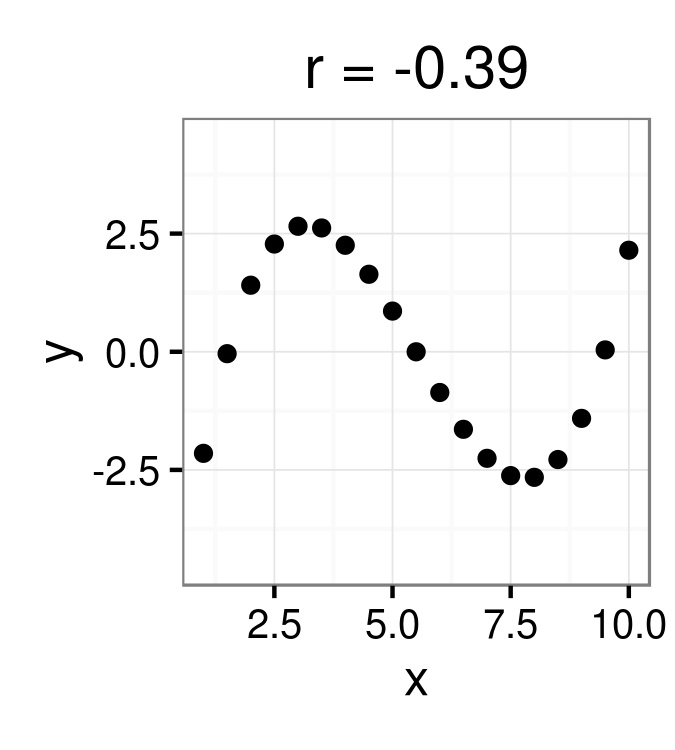
\includegraphics[width=2.25in]{../images/ch10_cor_cube}
\par}
\end{frame}

%%%%%%%%%%
\begin{frame}{``Real world" correlation}

{\centering
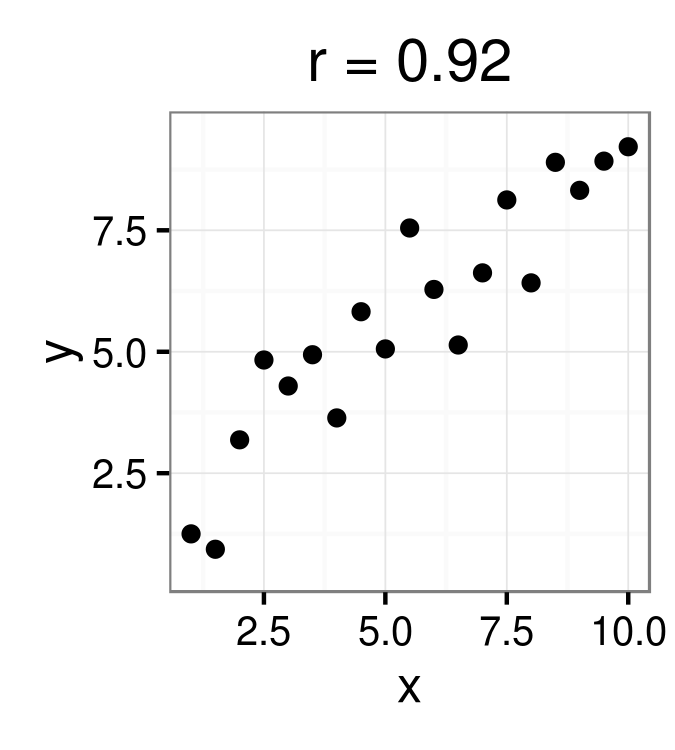
\includegraphics[width=2.25in]{../images/ch10_cor_pos3}
\pause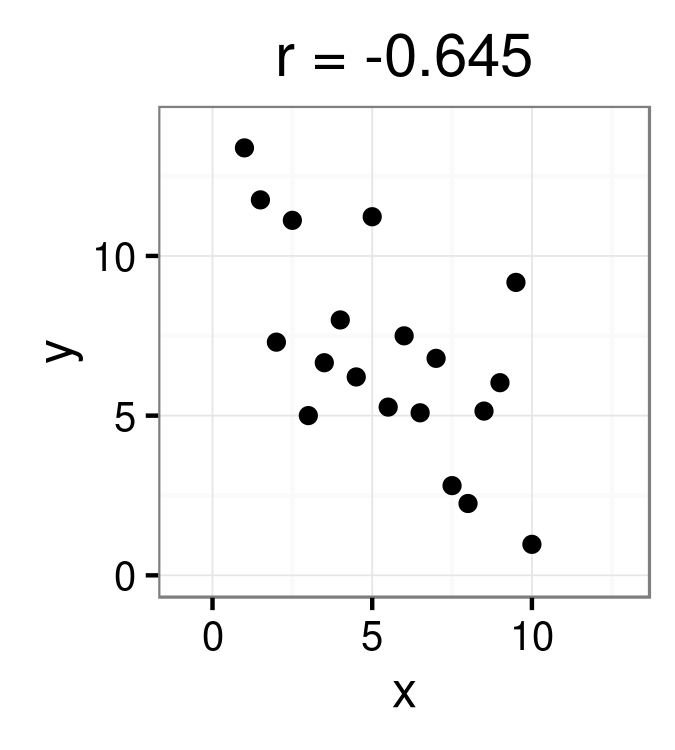
\includegraphics[width=2.25in]{../images/ch10_cor_neg3}
\par}
\end{frame}

%%%%%%%%%%
\begin{frame}{``Real world" correlation, cont.}

{\centering
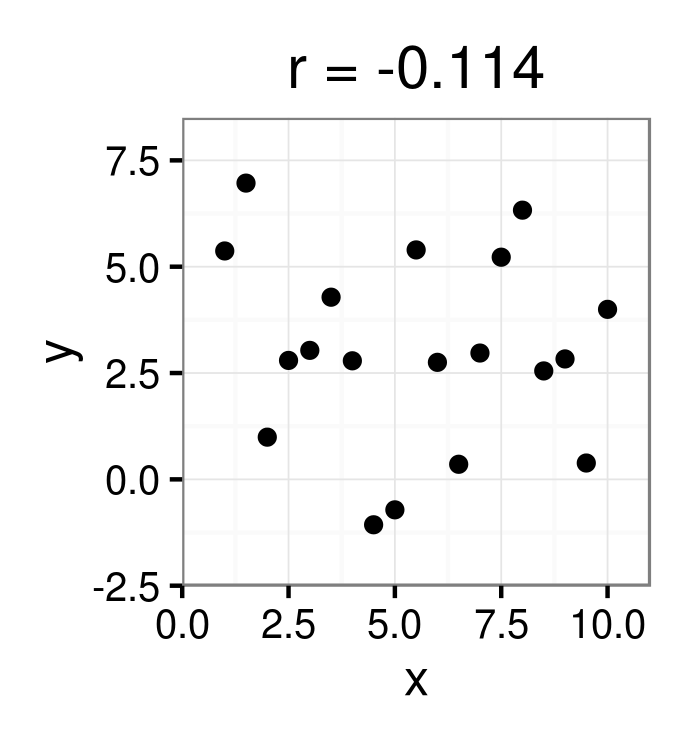
\includegraphics[width=2.25in]{../images/ch10_cor_zero2}
\par}
\end{frame}

%%%%%%%%%%
\begin{frame}{Correlation and outliers}
\begin{block}{}
The correlation coefficient $r$ is sensitive to outliers (very unusual values).
\end{block}
{\centering
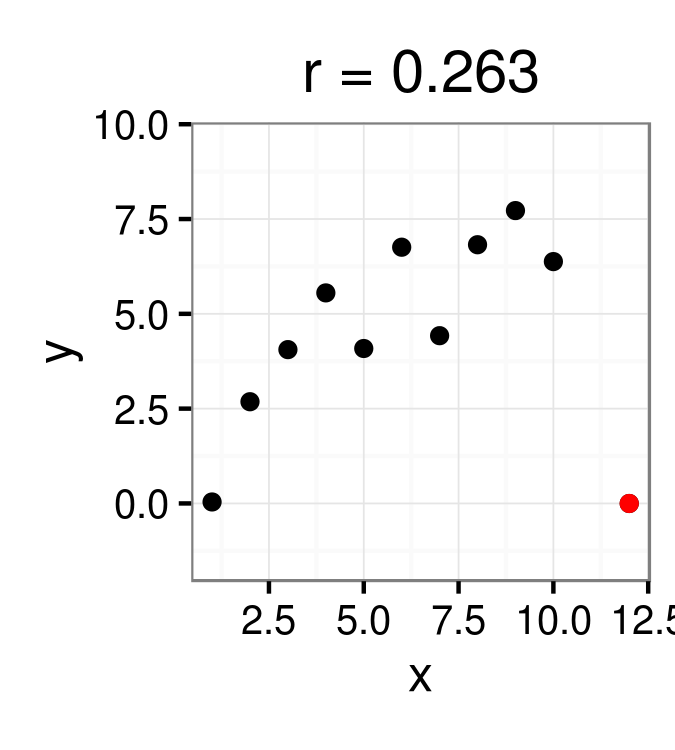
\includegraphics[width=2.25in]{../images/ch10_cor_w_out}
\pause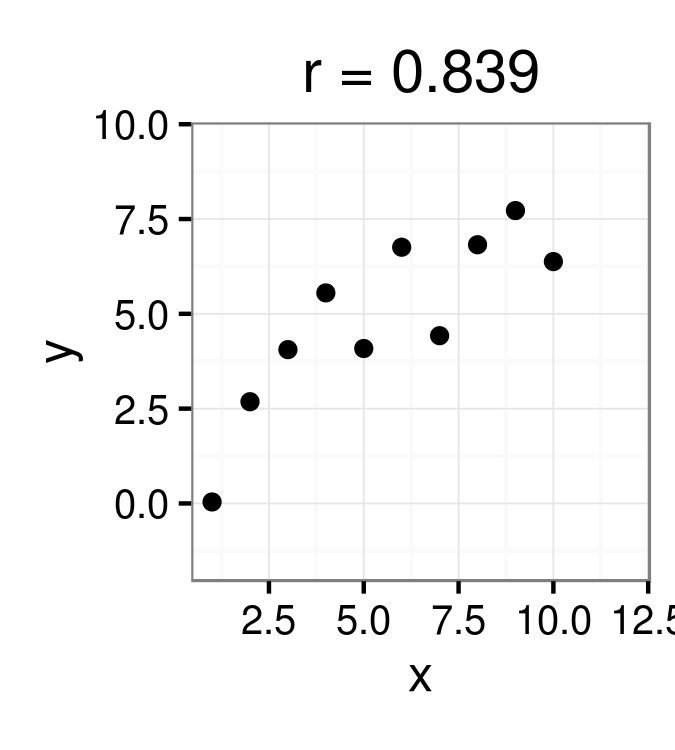
\includegraphics[width=2.25in]{../images/ch10_cor_wo_out}
\par}
\end{frame}

%%%%%%%%%%
\begin{frame}{Calculating correlation coefficient}
\begin{block}{}
To calculate $r$ one could use the following formula:\\
\medskip
\eq{r = \frac{n \Paren{\sum xy} - \Paren{\sum x}\Paren{\sum y}}
{\sqrt{n \Paren{\sum x^2} - \Paren{\sum x}^2}\sqrt{n \Paren{\sum y^2} - \Paren{\sum y}^2}}}
\medskip
\begin{itemize}
\pause\item While this formula will give you a value for $r$ (after much work), it doesn't help much in understanding how the correlation coefficient works. 
\pause\item Since technology should be used to calculate the correlation calculation anyway, it would be useful to look at $r$ defined with a more informative formula.
\end{itemize}
\end{block}
\end{frame}

%%%%%%%%%%
\begin{frame}{Calculating correlation coefficient, cont.}
\begin{block}{}
Consider: ($\propto$ means ``is proportional to")\\
\smallskip
\eq{r \propto \sum_{i=1}^n (x_i - \bar x) (y_i - \bar y)}
\begin{itemize}
\pause\item If when $x$ values are big (greater than $\bar x$) then $y$ values are big (greater than $\bar y$), and vice versa ($x < \bar x \to y < \bar y$), then $r$ is proportional to the sum of positive numbers, i.e. $r> 0$.
\pause\item If when $x$ values are big (greater than $\bar x$) then $y$ values are small (less than $\bar y$), and vice versa ($x < \bar x \to y > \bar y$), then $r$ is proportional to the sum of negative numbers, i.e. $r < 0$.
\pause\item If when $x$ values are far away from $\bar x$ then y values are also far away from $\bar y$ (whether positive or negative), then $r$ is proportional to the sum of larger numbers and will be closer to 1 or -1.
\end{itemize}
\end{block}
\end{frame}


%%%%%%%%%%
\begin{frame}{Correlation hypothesis tests}
\begin{block}{}
The sample correlation coefficient $r$ is an unbiased estimator for the population correlation coefficient $\rho$ (rho).\\
\medskip
Like population proportions and means, hypothesis tests can be conducted of the parameter $\rho$ to determine if a population of paired data is correlated.
\begin{itemize}
\pause\item $H_0: \rho = 0$
\pause\item $H_a: \rho \ne 0$\\ (It is uncommon to use the other forms of the alternative hypothesis)
\pause\item Test statistic: $\ds t= \frac r {\sqrt{\frac{1-r^2}{n-2}}} \qquad df = n-2$
\pause\item If $p < \alpha$, reject null hypothesis. There is evidence that the samples are correlated.
\end{itemize}
\end{block}
\end{frame}


%%%%%%%%%%
\begin{frame}{Strength of correlation}
\begin{block}{}
Even with statistically significant correlation, it might be useful to specify the strength of the correlation. While, like many things in statistics, the description of strength can be subjective and dependent of the context of the data, the following rule of thumb may be used:
\begin{itemize}
\pause\item $\Abs r \ge 0.7$ is a strong correlation
\pause\item $0.4 \le \Abs r < 0.7$ is a moderate correlation
\pause\item $\Abs r < 0.4$ is a weak correlation
\end{itemize}
\pause Thus, $r=0.5$ indicates a moderate positive correlation and $r=-0.8$ indicates a strong negative correlation.
\end{block}
\end{frame}


%%%%%%%%%%
\begin{frame}{Correlation, example}
\begin{exampleblock}{Example}
In 1886, Sir Francis Galton, a British sociologist, published the paper ``Regression towards Mediocrity in Hereditary Statures", in which he examined the heights of parents and their adult children. The core of modern uses of correlation and regression come from this paper (he also invented standard deviation). His data for fathers and sons is in the file ``Galton-father-son.csv" on D2L.\\
\medskip
Is there correlation between heights of fathers and their adult sons? Test at $\alpha = 0.05$ level of significance.
\begin{itemize}
\pause\item $H_0: \rho = 0$\\$H_a: \rho \ne 0$ 
\pause\item $r = 0.39131736$ \\ $p \ll 0.0001$
\end{itemize} 
\end{exampleblock}
\end{frame}

%%%%%%%%%%
\begin{frame}{Correlation, example}
\begin{exampleblock}{Example}
\begin{itemize}
\item $p < 0.0001 < \alpha = 0.5$. Reject null hypothesis
\item There is evidence that there is a correlation between the heights of fathers and their adult sons. However, $r < 0.4$ indicates weak correlation.
\end{itemize} 
\end{exampleblock}
\medskip
{\centering
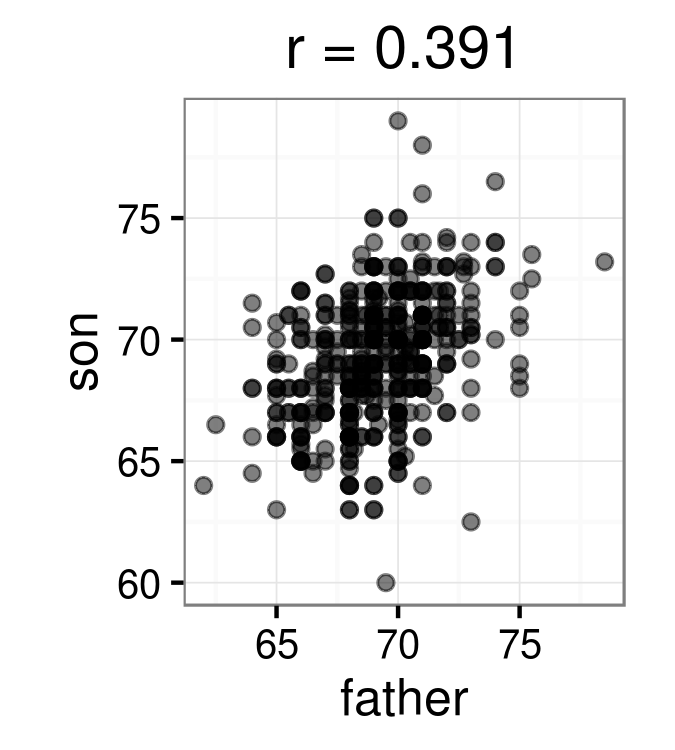
\includegraphics[width=1.6in]{../images/ch10_cor_galton}
\par}
\end{frame}

%%%%%%%%%%
\begin{frame}{Coefficient of determination}
\begin{block}{}
The \bt{coefficient of determination}, designated by $R^2$, represents the proportion of variation in one variable that is explained by the association with the other variable.
\begin{itemize}
\item The coefficient of determination is the correlation coefficient squared,  $R^2 = r^2$
\end{itemize}
\end{block}

\pause
\begin{exampleblock}{Example}
In the previous example, heights of fathers and sons had a correlation coefficient of $r=0.391$. Thus, $R^2 = (0.391)^2 = 0.153$.\\
\medskip
About 15\% of the variation of the heights of adult men can be explained by the association with their fathers heights.
\end{exampleblock}
\end{frame}

%%%%%%%%%%
\begin{frame}{Cautions}
\begin{block}{}
If a sample of paired data has a correlation coefficient that is zero or very low, that does not necessarily mean that there is not a association between the variables, only that there is not a \emph{linear} association. 
\end{block}

\pause
\begin{alertblock}{!!!}
\large
Correlation does not imply causation.
\end{alertblock}
\end{frame}

%%%%%%%%%%
\begin{frame}{Spurious correlations}
\begin{block}{}
From the \emph{Spurious Correlations} website:\\ \url{http://www.tylervigen.com/spurious-correlations}
\end{block}
\bigskip
{\centering
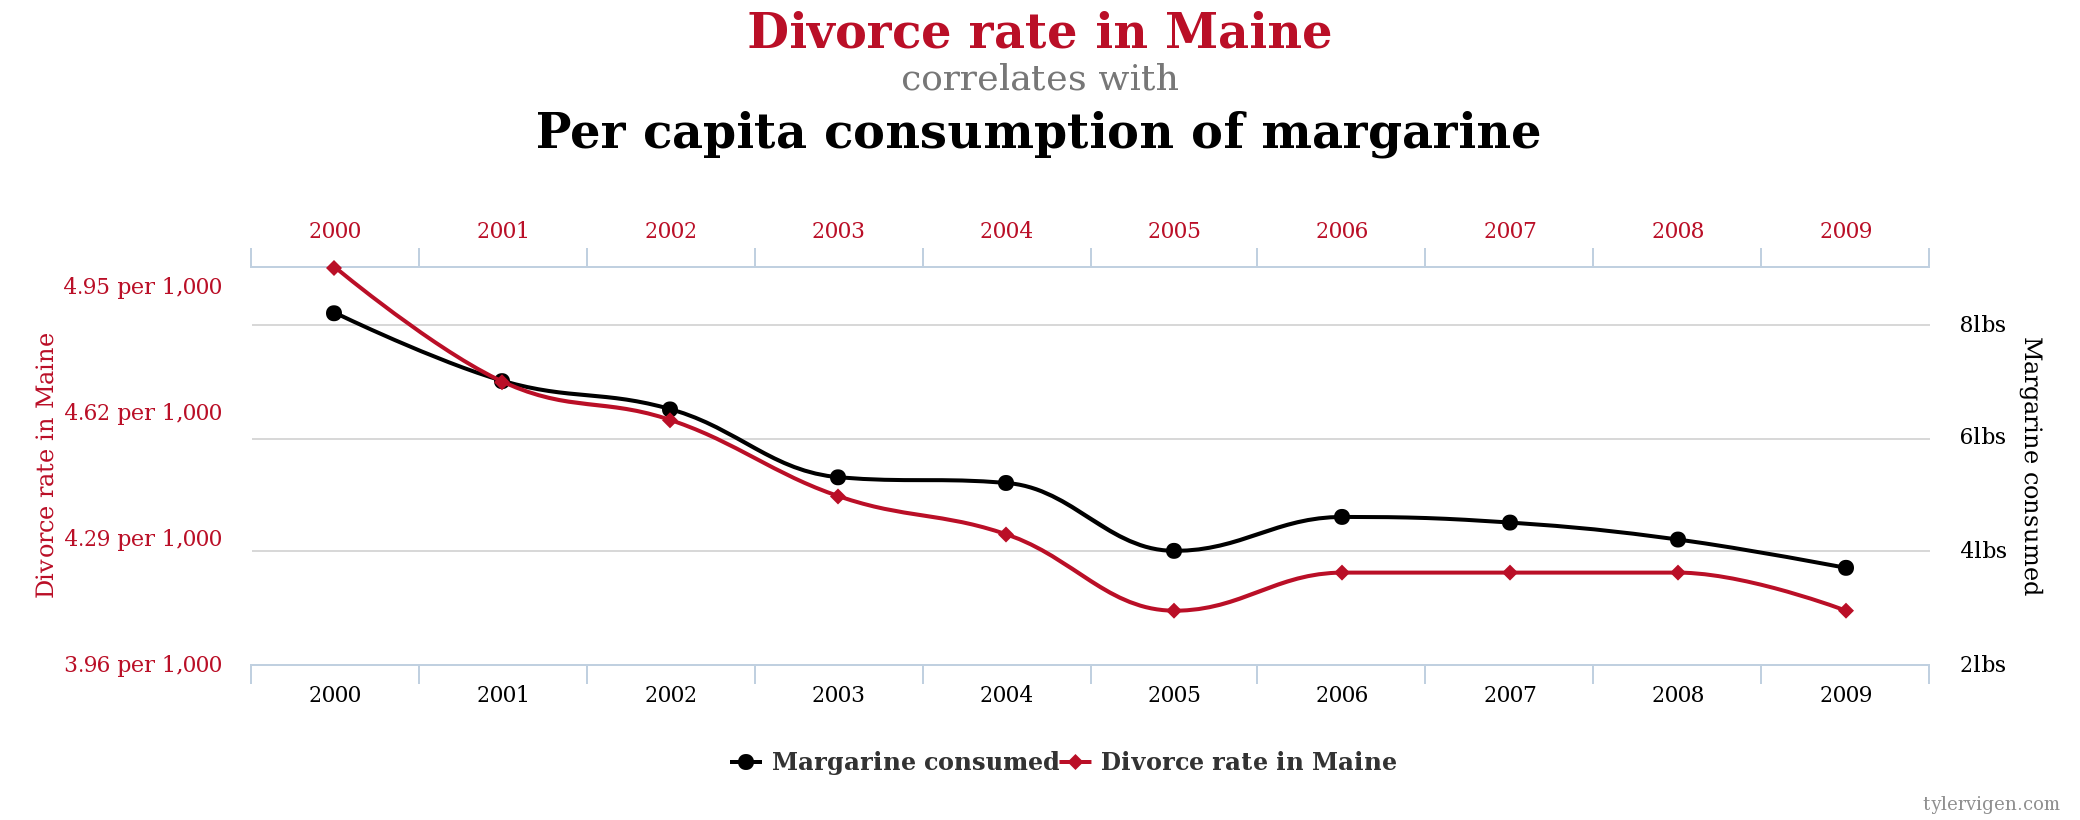
\includegraphics[width=4.75in]{../images/ch10_cor_spur}
\par}

\end{frame}

%%%%%%%%%%
\begin{frame}{Spurious correlations, cont.}
\bigskip
{\centering
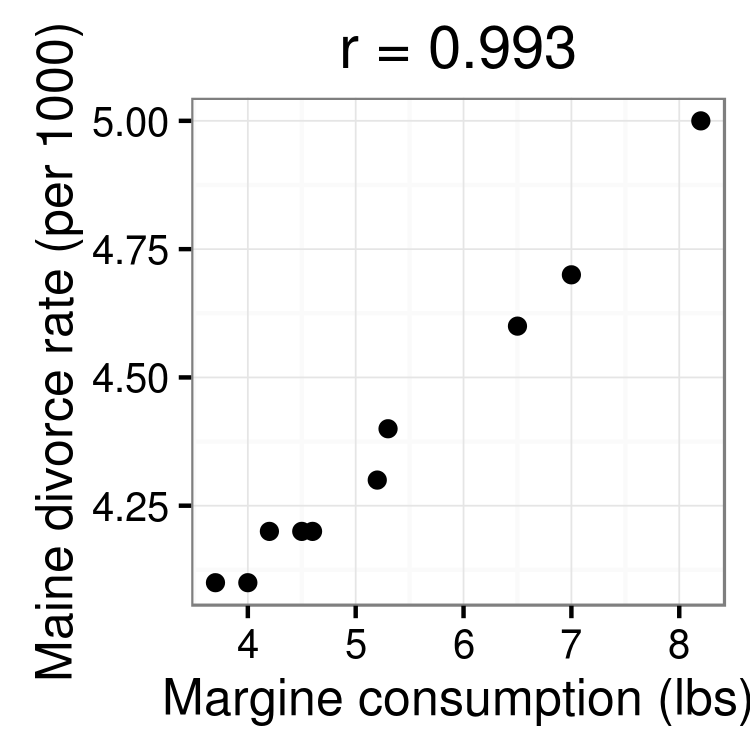
\includegraphics[width=2.5in]{../images/ch10_cor_spur2}
\par}

\end{frame}


%%%%%%%%%%
\begin{frame}{Correlation does not imply causation}

{\centering
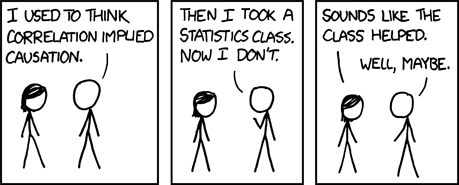
\includegraphics[width=4.5in]{../images/ch10_correlation}
\par}
\end{frame}

%%%%%%%%%%
%%%%%%%%%%
\begin{frame}<handout:0>{Group work}
\begin{block}{}
\begin{itemize}
\item For all the questions, complete parts (a) and (b).
\end{itemize}
\end{block}
\end{frame}

%
% Section 11.2
%
\subsection{Regression}

%%%%%%%%%%
\begin{frame}{Regression}
\begin{block}{}
Once it has been determined that two variables have a linear relationship, that is they have an association described by a straight line, the next logical question is what is that line.\\
\pause\medskip
\bt{Regression} is the statistical technique for finding the line that best describes a linear relationship between two paired variables.\\
\pause\medskip
The line found is known as the \bt{regression line} or the line of best fit.
\end{block}
\end{frame}

%%%%%%%%%%
\begin{frame}{Regression, example}

\medskip
{\centering
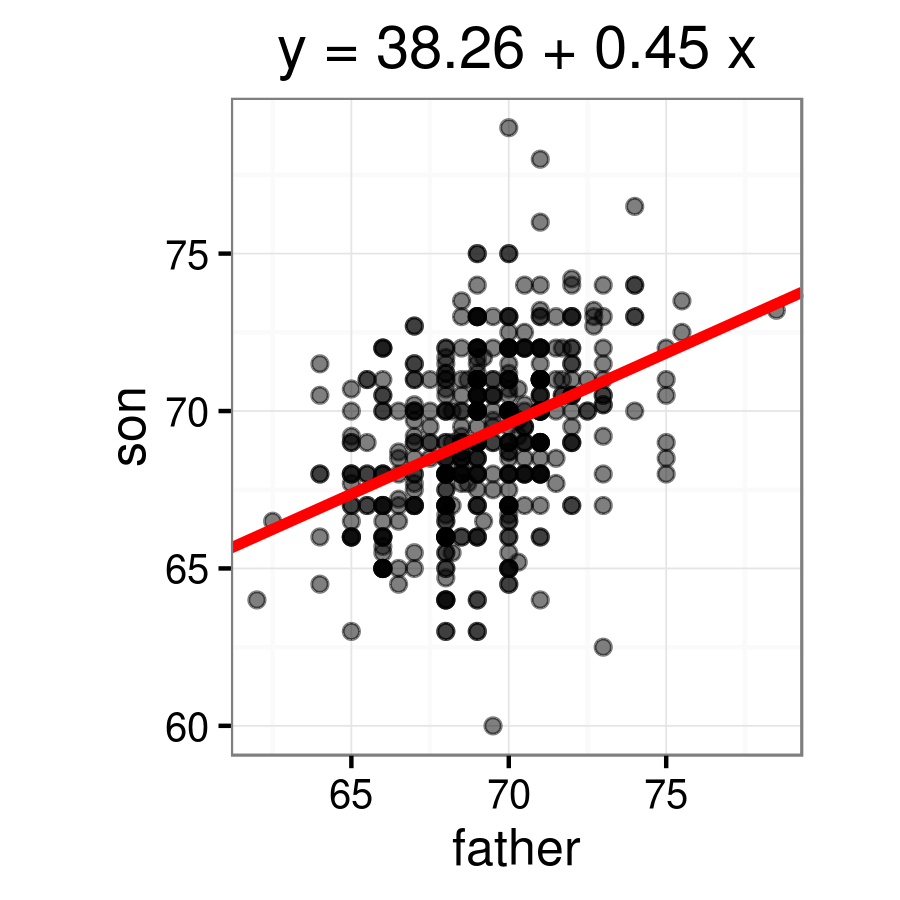
\includegraphics[width=2.8in]{../images/ch10_reg_galton}
\par}

\end{frame}

%%%%%%%%%%
\begin{frame}{Algebra review, lines}
\begin{block}{}
The equation for a line generally has the following form:\\
\smallskip
\eq{y = b + mx}
\begin{itemize}
\item $b$ is the $y$-intercept, or where the line crosses the y-axis ($x=0$).
\item $m$ is the slope of the line. It is the amount the $y$ value increases as the $x$ value increase by one.
\end{itemize}
\end{block}
\end{frame}

%%%%%%%%%%
\begin{frame}{Regression population models}
\begin{block}{}
A linear relationship between populations of variables $X$ and $Y$ can be described by:\\
\smallskip
\eq{Y = \beta_0 + \beta_1 X + \epsilon}
\smallskip
\begin{itemize}
\pause\item This equation is the \bt{model}, a possible structure for the relationship between the data.
\pause\item $X$ is known as the predictor variable, or the explanatory variable, or the independent variable.
\pause\item $Y$ is the response variable, or the dependent variable.
\pause\item $\beta_0$ and $\beta_1$ are the intercept and slope of a line describing the association of $X$ and $Y$.
\pause\item Like other population parameters, $\beta_0$ and $\beta_1$ are thought of as fixed, but unknown
\pause\item $\epsilon$ (epsilon) is a random error term. It is usually assumed that $\epsilon \sim N(0, \sigma^2)$.
\end{itemize}
\end{block}
\end{frame}

%%%%%%%%%%
\begin{frame}{Regression lines}
\begin{block}{}
The regression line for a sample paired data $(x,y)$ describes the linear relationship between $x$ and $y$. It is given by the equation:\\
\medskip
\eq{\hat y = b_0 + b_1 x}
\smallskip
\begin{itemize}
\pause\item $\hat y$ is the estimated $y$ value for a given $x$, or the predicted response.
\pause\item $b_1$, the slope of the regression line, is the amount of change in the predicted response for each unit increase in $x$
\pause\item $b_1$ can be calculated from the correlation coefficient, $\ds b_1 = r \frac{s_y}{s_x}$
\pause\item $b_0$, the $y$-intercept of the regression line, is usually not of much interest.
\end{itemize}
\end{block}
\end{frame}

%%%%%%%%%%
\begin{frame}{Hypothesis tests for regression}

\begin{block}{}
A simple linear regression model has two population parameters, $\beta_0$ and $\beta_1$, that are estimated by sample statistics, $b_0$ and $b_1$. As with other estimated parameters, an hypothesis test can be conducted to understand the population parameters. Generally, only the slope ($\beta_1$) is tested.

\begin{itemize}
\pause\item $H_0: \beta_1 = 0$
\pause\item $H_a: \beta_1 \ne 0$ \\ (this is most common, though the other forms can be used.)
\pause\item $b_1$ follows a $t$ distribution with $n-1$ degrees of freedom.
\pause\item This is the exact same test as the correlation test.
\end{itemize}

\end{block}
\end{frame}


%%%%%%%%%%
\begin{frame}{Predictions}
\begin{block}{}
If there is a valid regression equation ($\beta_1 \ne 0$), it can be used to make predictions of the response variable for given values of the predictor variable. Replace $x$ in the equation with the given predictor value and calculate the predicted response $\hat y$.
\end{block}

\pause
\begin{block}{}
However, if there is no correlation between values of paired data (if failed to reject null hypothesis for correlation test), then the best predictor for the response variable is simply $\bar y$.
\end{block}

\end{frame}

%%%%%%%%%%
\begin{frame}{Predictions, example}
\begin{exampleblock}{Example}
The regression line equation from the Galton data, for fathers height as predictor $x$ and sons height as response $y$, is \\
\smallskip
\eq{\hat y = 38.26 + 0.45 x}
\medskip
What is the predicted adult height of a son whose father is 68 inches tall?
\begin{itemize}
\pause\item $\hat y = 38.26 + 0.45 \times 68 = 68.86$ inches
\end{itemize}
\end{exampleblock}
\end{frame}

%%%%%%%%%%
\begin{frame}{Extrapolating}
\begin{block}{}
Predictions for predictor values outside the range of $x$ values used to find the regression line are highly suspect. This is known as \bt{extrapolating} and should be avoided.
\end{block}

\pause
\begin{exampleblock}{Example}
For the 2016-2017 season, NBA teams had field goal percentages between 43.5\% and 49.5\%. A regression line of the relationship between FG\% ($x$) and numbers of games won ($y$) is  \\
\eq{\hat y = -208.69 + 5.46 x}
\medskip
The GM for the Timberwolves wants to know how many games the team would win if they could get their FG\% up to 60\%, based on this data.
\begin{itemize}
\pause\item $\hat y = -208.69 + 5.46 \times 60 = 118.91$ games won
\end{itemize}

\end{exampleblock}

\end{frame}

%%%%%%%%%%
\begin{frame}{Extrapolating, example}

{\centering
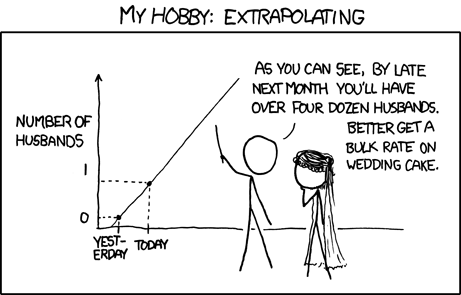
\includegraphics[width=4.5in]{../images/ch10_extrapolating}
\par}
\end{frame}



%%%%%%%%%%
\begin{frame}{Regression, example}
\begin{exampleblock}{Example}
The Department of Natural Resources wishes to track the weight of bears in the wild. While it is very difficult to weigh a bear, it is fairly easy to estimate the length of bear using photos. The data set ``bears.csv" on D2L contains measurements made from anesthetized wild bears.\\
\begin{itemize}
\item Find a relationship, if any, between the length and weight of bears using the data.
\item What is the best predicted weight of a bear thought to be 71 inches long?
\item Would it be appropriate to predict the weight of a bear 39 inches long? 89 inches?
\end{itemize}
\end{exampleblock}
\end{frame}

%%%%%%%%%%
\begin{frame}{Regression, example}

\smallskip
{\centering
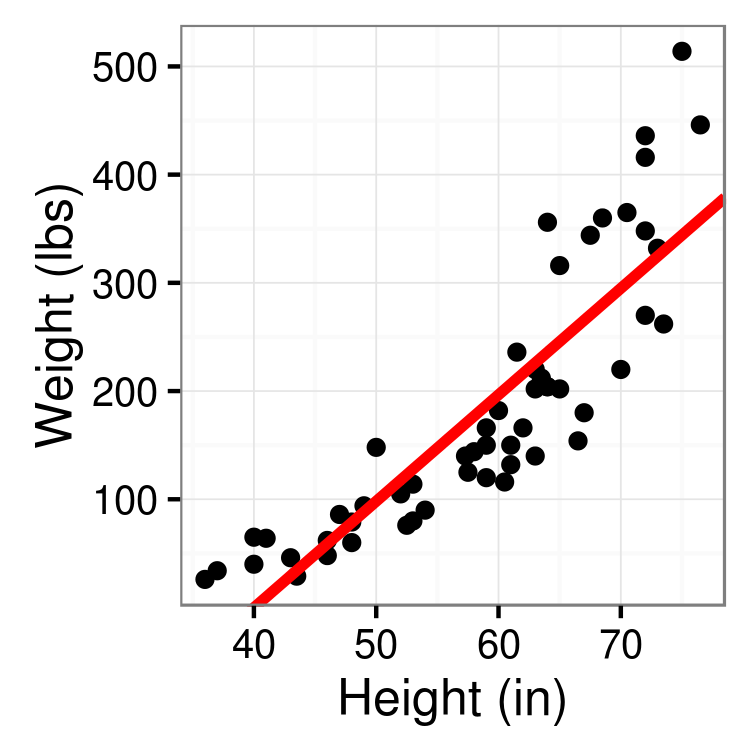
\includegraphics[width=2in]{../images/ch10_reg_bears}
\par}

\pause
\begin{exampleblock}{Example}
\begin{itemize}
\item $R^2 = 0.747$: About 75\% of the variation in bear weight is explained by the association with bear height.
\end{itemize}
\end{exampleblock}

\end{frame}

%%%%%%%%%%
\begin{frame}{Regression, example}
\begin{exampleblock}{Example}
\begin{itemize}
\item Regression line equation: $\hat y = -393.84 + 9.84 x$
\pause\item For every inch long a bear is, its weight will increase by about 10 lbs.
\pause\item A bear that is 71 inches long should weigh: \\
\eq{ \hat y = -393.84 + 9.84 \times 71= 304.7282 \text{ lbs.}}
\pause\item The $x$ values (bear length) used in the regression model are in the interval (36, 76.5). 
\pause\item Thus, it would be appropriate to predict the weight of a bear that is 39 inches long, but not a bear that is 89 inches long.
\end{itemize}
\end{exampleblock}

\end{frame}

%%%%%%%%%%
%%%%%%%%%%
\begin{frame}<handout:0>{Group work}
\begin{block}{}
\begin{itemize}
\item For all the questions, complete parts (c) and (d).
\end{itemize}
\end{block}
\end{frame}


\end{document}